% === Results ===
\section{Results}
\label{sec:results}

\subsection{RQ1: Retrieval Quality}
\label{sec:results-rq1}

Table~\ref{tab:retrieval} reports retrieval quality across all three datasets.
Two findings stand out. First, a retriever fine-tuned on the task far
outperforms strong off-the-shelf methods: our dense bi-encoder beats every
zero-shot dense embedder, classical lexical search, a cross-encoder re-ranker,
and a retrieval-augmented LLM on all three datasets: on real incidents it reaches \hit{5}~$0.91$ against $0.83$--$0.87$ for the best baselines.
The retrieval-augmented LLM, re-reading the same candidates, never surpasses it:
the gains come from domain-adapted retrieval, not a general reader.

\begin{table*}[t]
\centering
\caption{Retrieval quality on the held-out test set: Hit@1, Hit@5, and mean
reciprocal rank (MRR) under the coarse matching relation, averaged over the $n$ test
queries that have a ground-truth match. Best per column in \textbf{bold}. Our
fine-tuned dense retriever leads every zero-shot baseline and the
retrieval-augmented LLM on Hit@5 across all three datasets; hybrid fusion
additionally tops Hit@5 and MRR on the large real-world corpus (World of Logs),
where its Hit@5 gain over the dense retriever and the strongest baselines is
statistically significant (paired bootstrap, Benjamini--Hochberg $q<0.05$;
Fig.~\ref{fig:forest}). On the small synthetic corpora the dense retriever alone is
tied with or ahead of fusion.}
\label{tab:retrieval}
\footnotesize
\setlength{\tabcolsep}{4pt}
\begin{tabular}{l ccc ccc ccc}
\toprule
& \multicolumn{3}{c}{Online Boutique ($n{=}331$)}
& \multicolumn{3}{c}{OTel Demo ($n{=}119$)}
& \multicolumn{3}{c}{World of Logs ($n{=}5{,}150$)} \\
\cmidrule(lr){2-4}\cmidrule(lr){5-7}\cmidrule(lr){8-10}
Method & \hit{1} & \hit{5} & MRR & \hit{1} & \hit{5} & MRR & \hit{1} & \hit{5} & MRR \\
\midrule
\multicolumn{10}{l}{\emph{Prior art, zero-shot}}\\
\quad BGE (dense)          & 0.172 & 0.341 & 0.244 & 0.387 & 0.664 & 0.508 & 0.623 & 0.829 & 0.710 \\
\quad E5 (dense)           & 0.154 & 0.314 & 0.224 & 0.479 & 0.538 & 0.509 & 0.639 & 0.838 & 0.725 \\
\quad MPNet (dense)        & 0.202 & 0.375 & 0.278 & 0.227 & 0.630 & 0.404 & 0.644 & 0.834 & 0.725 \\
\quad TF--IDF (lexical)    & 0.127 & 0.372 & 0.231 & \textbf{0.521} & 0.613 & 0.563 & 0.521 & 0.766 & 0.626 \\
\quad Cross-encoder rerank & 0.103 & 0.296 & 0.182 & 0.311 & 0.580 & 0.441 & 0.686 & 0.874 & 0.766 \\
\multicolumn{10}{l}{\emph{Retrieval-augmented LLM}}\\
\quad Qwen2.5-7B           & 0.239 & 0.344 & 0.293 & 0.370 & 0.639 & 0.501 & 0.710 & 0.856 & 0.778 \\
\multicolumn{10}{l}{\emph{Ours}}\\
\quad Dense bi-encoder     & \textbf{0.432} & \textbf{0.634} & \textbf{0.512} & 0.445 & \textbf{0.681} & 0.549 & \textbf{0.856} & 0.905 & 0.874 \\
\quad Knowledge graph      & 0.396 & 0.465 & 0.420 & 0.067 & 0.412 & 0.227 & 0.083 & 0.308 & 0.152 \\
\quad Hybrid fusion        & 0.414 & 0.559 & 0.461 & 0.513 & 0.672 & \textbf{0.568} & 0.839 & \textbf{0.970} & \textbf{0.897} \\
\bottomrule
\end{tabular}
\end{table*}

Second, the value of \emph{fusion} depends on the setting. On the large,
heterogeneous real corpus, fusing the dense, sparse, and graph retrievers lifts
\hit{5} from $0.91$ to $0.97$, placing the correct prior incident in the top
five $97\%$ of the time, at \hit{1}~$0.84$ and MRR~$0.90$. This gain is large and
statistically significant: against the dense retriever the paired-bootstrap
difference is $+0.065$ ($95\%$ CI $[+0.058,+0.073]$), and against the strongest
baselines it ranges from $+0.12$ (the LLM) to $+0.14$ (zero-shot dense), all with
Benjamini--Hochberg $q\approx 0$. On the two small synthetic corpora, by
contrast, the fine-tuned dense retriever is already so strong that fusion does
not help, and on Online Boutique it is slightly worse ($-0.076$, $q=0.03$):
when one retriever dominates a small memory, blending in weaker signals only adds
noise. Fusion's advantage thus \emph{emerges with scale and diversity}, precisely
the conditions of real operations. Figure~\ref{fig:forest} summarizes every
pairwise comparison with its bootstrap confidence interval and significance.

\begin{figure}[t]
\centering
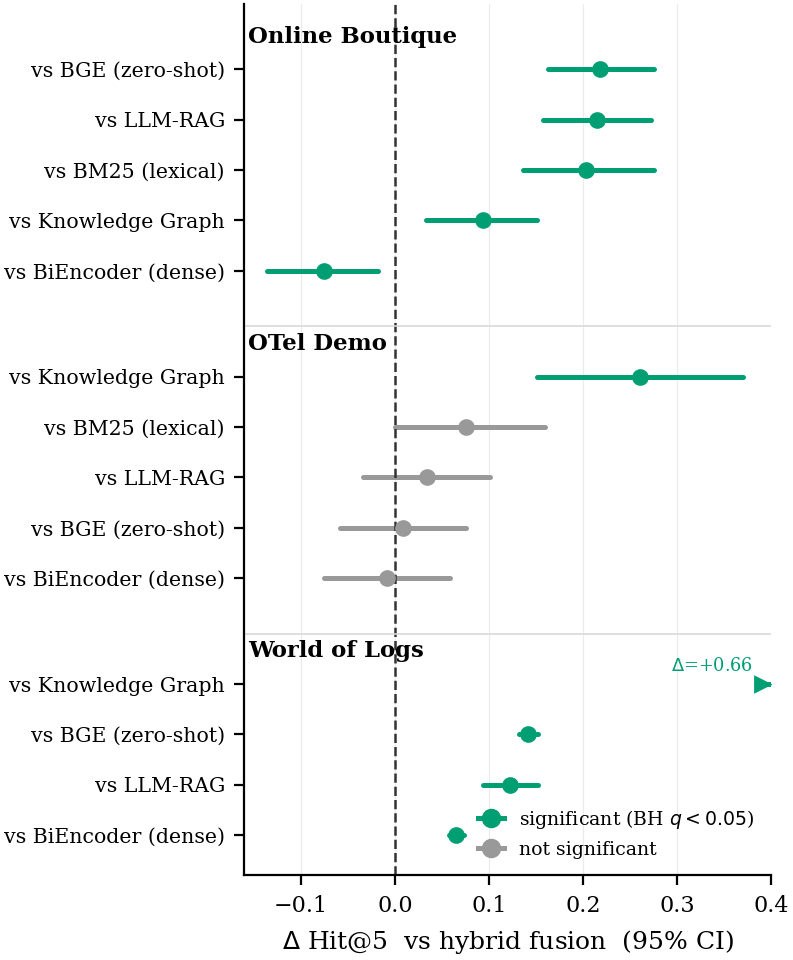
\includegraphics[width=0.82\columnwidth]{figures/fig_significance_forest.png}
\caption{Difference in \hit{5} between hybrid fusion and each alternative (paired
bootstrap, $95\%$ CI; green = significant after Benjamini--Hochberg). Hybrid wins
decisively on real data (WoL) and beats the graph baseline on every dataset; on
the small synthetic corpora it ties or trails the fine-tuned dense retriever.}
\label{fig:forest}
\end{figure}

\subsubsection*{The stricter relation, and what the numbers are worth}
\label{sec:results-strict}

The coarse relation is permissive, and we think the honest way to present it is
alongside both a stricter relation and a reference point for what the scores
mean. Table~\ref{tab:strict} reports every method we have per-query predictions
for under the strict relation, which additionally demands substantial symptom
overlap.

Two calibration facts frame the table. First, the relations differ greatly in how
much of memory they admit: the average query has $288$ relevant items under the
coarse relation ($0.75\%$ of the $38{,}642$-item memory) but only $34.5$ under the
strict one ($0.09\%$). Second, the corresponding expected \hit{5} for a uniformly
random ranker is therefore $0.036$ coarse and $0.0044$ strict. Hybrid retrieval's
$0.970$ and $0.744$ sit $27\times$ and $169\times$ above those references.

Under the strict relation hybrid fusion remains best on all three metrics against
every system we could test pairwise, and the margins survive correction: $+0.038$
\hit{5} over BGE ($95\%$ CI $[+0.025,+0.051]$), $+0.050$ over the cross-encoder
($[+0.038,+0.064]$), and $+0.221$ over our own dense retriever
($[+0.206,+0.237]$), all with Benjamini--Hochberg $q<0.001$. The single exception
is \hit{5} against raw-corpus BM25 ($+0.004$, $[-0.011,+0.019]$, $q=0.54$); that
method's \hit{1} of $0.015$ reflects a degenerate top-rank ordering, and hybrid
beats it on MRR by $+0.271$. The result also holds across \emph{both} held-out
project domains (Kafka~$0.80$, MariaDB~$0.73$).

One result in Table~\ref{tab:strict} deserves emphasis because it cuts against
our own method. Our fine-tuned dense retriever, which is trained against the
coarse relation, is the \emph{largest} loser under the strict one, falling from
$0.905$ to $0.523$ and dropping below every zero-shot embedder. Fusion does not:
it falls from $0.970$ to $0.744$ and stays on top. We read this as evidence that
the evaluation is not simply rewarding methods aligned with the labelling rule
(\S\ref{sec:results-leakage}), since the component most aligned with that rule
degrades the most.

\begin{table}[t]
\centering
\caption{Retrieval on World of Logs under the \emph{strict} relation (coarse
$+$ symptom-token overlap), on the $n{=}4{,}362$ held-out queries that retain a
gold match under it. Best per column in \textbf{bold}. A uniformly random ranker
would score \hit{5}~$0.0044$ here. The fine-tuned dense retriever, trained
against the coarse relation, degrades most; fusion holds up.}
\label{tab:strict}
\footnotesize
\setlength{\tabcolsep}{5pt}
\begin{tabular}{lccc}
\toprule
Method & \hit{1} & \hit{5} & MRR \\
\midrule
\multicolumn{4}{l}{\emph{Prior art, zero-shot}}\\
\quad BGE (dense)          & 0.474 & 0.706 & 0.564 \\
\quad E5 (dense)           & 0.450 & 0.698 & 0.544 \\
\quad TF--IDF (lexical)    & 0.445 & 0.715 & 0.559 \\
\quad BM25 (raw corpus)    & 0.015 & 0.740 & 0.332 \\
\quad Cross-encoder rerank & 0.418 & 0.694 & 0.523 \\
\multicolumn{4}{l}{\emph{Ours}}\\
\quad Dense bi-encoder     & 0.260 & 0.523 & 0.356 \\
\quad Knowledge graph      & 0.016 & 0.036 & 0.023 \\
\quad Hybrid fusion        & \textbf{0.511} & \textbf{0.744} & \textbf{0.602} \\
\bottomrule
\end{tabular}
\end{table}

We isolated the graph's contribution by comparing fusion with and without it. It surfaces correct candidates the
others miss (on $14\%$ of Online Boutique queries it retrieves the right
incident where the dense retriever fails), but in fusion this rarely changes
top-five recall (the $\pm$graph difference is not significant on any dataset).
The graph is therefore a real but marginal contributor: useful for top-rank
precision and coverage, not a driver of \hit{5}.

\subsubsection*{Does the relevance rule leak into the retrievers?}
\label{sec:results-leakage}

The coarse relation is defined on a ticket's Jira \texttt{components} metadata,
and our graph retriever scores candidates partly by component overlap. That
coincidence invites a serious objection: perhaps the headline reflects the
labelling rule rather than retrieval quality. We take it seriously and report
four independent checks, three of which we ran specifically to test it.

\emph{(i) The retrievers never see the field.} The indexed corpus is built from
ticket narrative and pasted log and code blocks only. Sampling $3{,}000$ indexed
memory documents, \emph{none} contains a \texttt{Components} field, and only
$34.6\%$ of gold component names appear anywhere in the indexed text at all, as
incidental prose mentions. On the query side the figure is $15.9\%$. (A legacy
composed-text file in our data release does embed the field verbatim; it is not
what is indexed, and we exclude it from the published bundle to prevent a reader
from reproducing against it by mistake.)

\emph{(ii) The graph's vocabulary barely overlaps the gold vocabulary.} Graph
entities are extracted from ticket text by a language model, not read from
metadata. Over the $38{,}600$ memory extractions the extracted component
vocabulary has $1{,}559$ distinct terms and the gold vocabulary $1{,}101$; they
share $109$, or $9.9\%$ of the gold vocabulary. Roughly nine in ten terms that
define relevance never enter the graph.

\emph{(iii) The graph retriever is the worst system, not the best.} If the rule
leaked through it, it would dominate. It is last under both relations (coarse
\hit{5}~$0.308$, strict $0.036$), and removing it from fusion changes \hit{5}
significantly on no dataset.

\emph{(iv) The component most aligned with the rule degrades the most.} As noted
above, our dense retriever is fine-tuned against the coarse relation and loses
most under the strict one ($0.905\!\rightarrow\!0.523$), while fusion holds up
($0.970\!\rightarrow\!0.744$). An evaluation rigged toward our method would not
behave this way.

None of this makes the coarse relation a measure of diagnostic usefulness, which
it is not (\S\ref{sec:threats}); it addresses only the narrower question of
whether the labelling rule leaks into the systems being compared. We find no
evidence that it does.

\smallskip
\noindent\textbf{How much does the training seed matter?} Retriever fine-tuning
is the only stochastic step in the pipeline (\S\ref{sec:setup-protocol}), so we
quantify its contribution rather than assume it away. Retraining under five
seeds leaves coarse \hit{5} at $0.636\pm0.016$ on Online Boutique and
$0.676\pm0.005$ on OTel Demo (mean $\pm$ sample standard deviation), so the lead
over the zero-shot embedders is not an artifact of a lucky initialization.

Decomposing that variability against the other source, sampling of the test
queries, shows the two datasets behave quite differently. On OTel Demo the seed
standard deviation ($0.005$) is dwarfed by the query-bootstrap standard deviation
($0.044$) and contributes about $1\%$ of the total variance; there, a single run
is defensible. On Online Boutique the two are comparable ($0.016$ versus
$0.026$), with the seed accounting for roughly $28\%$ of the variance, so an
interval computed from query resampling alone understates the true uncertainty.
We therefore report seed-aware intervals, $\sqrt{\sigma^2_{\text{seed}}+
\sigma^2_{\text{sample}}}$, wherever a retrained component is compared.

We note two things about the magnitude. Top-1 is markedly less stable than
top-5 on Online Boutique (\hit{1} spans $0.417$--$0.468$ across seeds, a range of
$0.051$, against $0.039$ for \hit{5}), so single-seed \hit{1} comparisons on the
small corpora deserve particular caution. And the largest full seed-to-seed range
we observe anywhere is $0.039$, against which the real corpus's headline margin
of $+0.065$ \hit{5} over the dense retriever is a factor of $1.7$ larger.

\subsection{RQ2: End-to-End Triage and Graceful Degradation}
\label{sec:results-rq2}

Table~\ref{tab:agent} reports the full end-to-end system. The headline is
robustness across evidence regimes: the \emph{same} system, with no
reconfiguration, retrieves strongly whether it has complete telemetry or only text,
reaching \hit{5}~$0.96$ on the real, text-only incidents (essentially realizing the
hybrid retriever's quality end to end) and $0.76$ on the fully instrumented
synthetic systems.

Duplicate suppression fires where there are duplicates to suppress, and we report
it as a rate rather than as pages per incident, which our harness makes $1.0$ by
construction. On the real corpus, $3{,}061$ of $10{,}566$ would-be pages
($29.0\%$) are folded into an incident already raised. The telemetry corpora give
it far less to do ($5.3\%$ and $0.9\%$), since their scenarios are short and
rarely span many consecutive ticket-worthy windows; the mechanism is therefore
exercised meaningfully only on the real corpus, and we do not claim it as
validated on the synthetic ones.

Triage accuracy tells a different story across regimes. On the telemetry datasets
the system clears the majority-class baseline by a useful margin ($0.841$ against
$0.784$, and $0.846$ against $0.725$). On the real corpus it reaches $0.506$
against a $0.506$ baseline, i.e.\ no better than always predicting the majority
class. We say this plainly: our own end-to-end triage on real incidents carries
no usable signal either, which is consistent with, not an exception to, the
reframing in \S\ref{sec:results-rq4}.

One might suspect this is an artifact of page suppression, which re-labels a
suppressed window \emph{borderline}, a class the binary resolution-derived gold
cannot match. It is not. The harness scores triage on the pre-suppression
decision precisely to avoid charging a paging action as a triage error, and the
effect is verifiable: a configuration with suppression disabled, which emits no
borderline decisions at all, classifies exactly the same $6{,}769$ of $13{,}388$
windows correctly as the configuration that suppresses $3{,}061$ pages. The
$0.506$ is therefore a genuine absence of signal, not a scoring artifact.

\begin{table}[t]
\centering
\caption{End-to-end system (RQ2) and the cost saved by capability gating (RQ3),
per dataset. Triage accuracy is reported against the majority-class baseline,
which it does not beat on the real corpus. Duplicate suppression is given as the
share of would-be pages folded into an existing incident; we do not report pages
per incident, which is $1.0$ by construction in our harness and therefore
uninformative. Cost saving is an \emph{estimated} counterfactual: gate decisions
priced with a fixed per-skill cost model (\S\ref{sec:results-rq3}), not a
measured wall-clock comparison.}
\label{tab:agent}
\footnotesize
\setlength{\tabcolsep}{5pt}
\begin{tabular}{lccc}
\toprule
 & Online Boutique & OTel Demo & World of Logs \\
\midrule
\hit{1}                        & 0.689 & 0.647 & 0.859 \\
\hit{5}                        & 0.758 & 0.756 & 0.963 \\
MRR                            & 0.714 & 0.688 & 0.902 \\
Triage accuracy                & 0.841 & 0.846 & 0.506 \\
\quad\emph{majority baseline}  & \emph{0.784} & \emph{0.725} & \emph{0.506} \\
Would-be pages suppressed      & 5.3\% & 0.9\% & 29.0\% \\
\midrule
Cost saved (gating, estimated) & 40\%  & 63\%  & 78\% \\
\bottomrule
\end{tabular}
\end{table}

\subsection{RQ3: The Cost of Adaptive Execution}
\label{sec:results-rq3}

What does the capability-gated controller buy? Running only the steps the
evidence supports, and escalating expensive steps only under uncertainty,
reduces per-window cost by $40\%$, $63\%$, and $78\%$ on the three datasets
relative to a cascade that runs everything (Table~\ref{tab:agent}).

We are precise about what that figure is and is not. The \emph{counts} are
measured: we log per window which skills ran and which a gate skipped
($75{,}334$ invocations and $31{,}734$ gate skips on the real corpus). The
\emph{per-call unit costs} are modelled, from a fixed table released with the
artifact. The reported percentage is counts $\times$ modelled units, so calling
it a measured wall-clock reduction, as our earlier phrasing did, overstates it.

The natural objection is that the conclusion then rests on the cost table. It
does not, and the reason is structural. Every gated skill sits behind the
\emph{same} escalation gate, so each is skipped at nearly the same rate; the
saving therefore approximates that gate's closure rate almost independently of
what the individual skills cost. Recomputing the entire saving with each skill's
\emph{measured} mean duration as its unit cost, instead of the modelled one,
gives $79.0\%$ against the modelled $77.9\%$, a difference of $1.1$ points, even
though the table misprices individual skills badly (it overstates query
reformulation by three orders of magnitude and understates the peer-incident
lookup, the only step doing real I/O, by $68\times$). Varying the verifier's
assumed per-call cost between $0.5\times$ and $2\times$ moves the real-corpus
figure not at all, since that skill is disabled there.

What the figure does \emph{not} capture is equally important: this evaluation
harness replays precomputed predictions, so its measured end-to-end wall-clock
($43$\,ms per window) is the cost of replaying a decision, not of making one. We
therefore report cost as an explicitly modelled counterfactual rather than as a
deployment measurement, and treat the gate-closure rates as the quantity the
result actually rests on. Those rates are what differ across datasets: the $78\%$
on the real corpus reflects reformulation being skipped on $10{,}566$ of
$13{,}376$ windows, and the telemetry figures reflect the evidence tools being
skipped on $41\%$ and $65\%$. The saving does not "grow with scale" so much as
track how often each deployment's dominant gate closes.

This thrift costs no accuracy: an ablation that
removes each component in turn moves \hit{1} by at most $0.012$, and sweeping the
evidence-gathering budget leaves \hit{5} unchanged. The same measurements carry a candid message: no single component is load-bearing, so the heavyweight evidence-gathering tools add little measurable \hit{} gain here; they keep cost low by running only when cheaper steps are unsure, and their headroom is bounded by how often retrieval is already correct.

\smallskip
\noindent\textbf{Where the gate thresholds sit.} Because the escalation decision
is driven by a threshold on $\mathrm{maxconf}$ (Eq.~\ref{eq:maxconf}), its value
deserves a sensitivity analysis rather than an assertion. Using the per-window
counterfactual between the cheap-path-only and full-stack configurations, we
sweep a unified escalation threshold over the realized confidence distribution on
the real corpus (Table~\ref{tab:threshold}). Escalation is worth $+0.059$ \hit{5}
in aggregate ($0.904\!\rightarrow\!0.963$), but the curve saturates early: a
threshold of $0.477$ already reaches the full-escalation quality of $0.963$ while
escalating three quarters of windows, and $0.362$ retains $0.935$ while escalating
only a quarter. The shipped $0.5$ is thus on the saturated plateau, buying no
additional quality over $0.477$ at a higher escalation rate. On the telemetry
datasets the sweep is flat at every threshold, consistent with the finding above
that the expensive path never changes their rankings.

\begin{table}[t]
\centering
\caption{Escalation-threshold sensitivity on World of Logs ($n{=}5{,}150$). A
window escalates when its cheap-path confidence falls below the threshold.
Quality saturates well before the shipped operating point.}
\label{tab:threshold}
\footnotesize
\setlength{\tabcolsep}{5pt}
\begin{tabular}{cccl}
\toprule
Threshold & Windows escalated & \hit{5} & \\
\midrule
$0.000$ & \phantom{0}0.0\% & 0.904 & (never escalate) \\
$0.293$ & \phantom{0}5.0\% & 0.911 & \\
$0.362$ & 25.0\% & 0.935 & \\
$0.400$ & 41.8\% & 0.955 & \\
$0.450$ & 61.0\% & 0.963 & \\
$0.477$ & 75.0\% & 0.963 & cheapest to match full escalation \\
$0.500$ & 85.4\% & 0.963 & shipped operating point \\
$0.600$ & 100.0\% & 0.963 & (always escalate) \\
\bottomrule
\end{tabular}
\end{table}

\smallskip
\noindent The ablation isolates one capability that sits apart from retrieval rank,
\emph{novelty detection}: removing the novelty-composition step leaves \hit{5}
unchanged but drops recall of novel, no-precedent incidents from $0.54$ to $0$ on
Online Boutique, so the step is load-bearing for flagging failures with no
precedent even though it never moves top-five retrieval. On the text-only real
corpus this flag is confounded with ordinary retrieval uncertainty (weakening
retrieval only makes more windows look novel), so we report novelty on the
synthetic telemetry data alone.

\begin{figure*}[t]
\centering
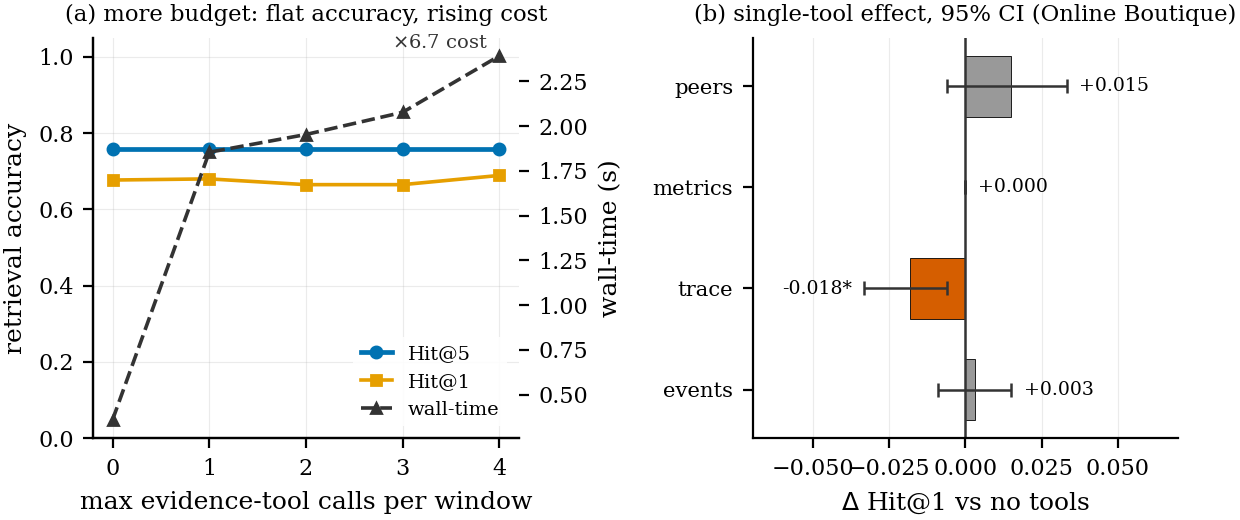
\includegraphics[width=.8\textwidth]{figures/fig_adaptive_execution.png}
\caption{Adaptive execution on the fully-instrumented Online Boutique system
(RQ3). (a)~Raising the evidence-gathering budget leaves retrieval accuracy
unchanged (\hit{5} flat at $0.76$; \hit{1} within a $0.024$ band) while wall-clock
time grows $6.7\times$: more budget buys latency, not accuracy. (b)~Single-tool
effect on \hit{1} with $95\%$ paired-bootstrap confidence intervals ($1{,}000$
resamples, the same procedure as Fig.~\ref{fig:forest}); $*$ marks an interval
excluding zero. \emph{No evidence tool has a demonstrable benefit}: the
peer-incident lookup, the largest positive point estimate, is
$+0.015$ with CI $[-0.006,+0.033]$. Only the extended-trace reader has a
demonstrable effect and it is \emph{harmful} ($-0.018$, CI $[-0.033,-0.006]$),
and only when it runs alone: added alongside the peer lookup the effect falls to
$-0.003$ (CI $[-0.009,+0.000]$, n.s.). On OTel Demo and World of Logs every tool
effect is identically $0.000$. The controller's value is therefore to invoke
these tools only when cheaper steps are unsure, not to add accuracy.}
\label{fig:adaptive}
\end{figure*}

\subsection{RQ4: Synthetic Versus Real, and What It Reveals}
\label{sec:results-rq4}

Our most consequential finding concerns the triage \emph{classification} task
that dominates synthetic benchmarks, deciding whether a window is ticket-worthy
at all. On synthetic data it is trivially easy: standard classifiers over the
telemetry features reach a near-perfect area under the precision--recall curve
(ROC area $1.00$) and are well calibrated.

Real incidents carry no telemetry features, so the comparison must be made on
the input that corpus actually has, its text. Under the identical
leave-domain-out protocol and five seeds, a TF--IDF linear model reaches ROC
area $0.601$ ($95\%$ CI $[0.592,0.611]$), gradient boosting over a truncated-SVD
projection $0.583$, and logistic regression $0.572$. The intervals exclude
$0.50$, so real-incident text does carry signal, but the task retains only a
small fraction of what injected telemetry offers, and at the operating threshold
the gain over the majority-class baseline ($0.506$) is slight. The near-perfect
synthetic number is thus an artifact of fault injection, where active faults are
separable from baselines by construction, rather than evidence that
ticket-worthiness is an easy prediction on real, engineer-written tickets. We further confirm that the synthetic signal is
genuine rather than memorized: on Online Boutique we inject \emph{orphan} faults,
real ticket-worthy failures deliberately left with no matching ticket in memory, and
the triage classifiers flag them as reliably as the reported faults (recall gap
within $5$ points, and $1.00$ versus $1.00$ for the gradient-boosted model), so the
near-perfect synthetic number reflects fault-versus-baseline separability, not
memorization of which incidents carry tickets. This check is informative only there:
the other telemetry set contained no orphan faults, and on the real corpus triage is
already weak.

The real-data conclusion is not an artifact of how we binarize the three-way
label. Dropping the ambiguous \emph{borderline} class and classifying
ticket-worthy against noise alone raises the best text model to ROC area $0.704$
($95\%$ CI $[0.688,0.721]$) on $8{,}024$ held-out issues, still far below the
synthetic $1.00$ and still at the majority-class accuracy ($0.844$). Both
binarizations agree: real-incident text carries measurable but weak
ticket-worthiness signal.

This reframes how operational triage should be measured: the part that looks solved on synthetic data does not transfer, while the part that does (retrieving which past incident a live one resembles) is where the real headroom lies, and where our system is strongest.

Because the real dataset's matches are inferred rather than human-labelled, we
probed them with an LLM-as-judge. Asked to rate each gold match against a control,
the judge separates the two on every dataset, most sharply on the real incidents
(a gold-versus-control gap of $1.24$ on a five-point scale, versus $0.34$--$0.47$
on synthetic). The same run, however, qualifies what that gap establishes: only
$6.3\%$ of coarse-gold matches are rated $4$ or $5$, against $0\%$ of controls. So
the judge finds the relation clearly non-random, but it does \emph{not} find most
coarse-gold pairs to be strongly related. Together with the controls being
uniformly sampled, and therefore easy, this check should be read as evidence that
the coarse relation captures topical relatedness, not that it identifies the
prior incident an engineer would most want. We report the strict relation
(\S\ref{sec:results-strict}) for that reason, and a human study remains the
right instrument (\S\ref{sec:threats}).